\section{Task 7: Optional Challenges}
\subsection{a)}

\subsection{b)}

\subsection{c)}

\subsection{d)}

\subsection{e)}
See \cref{fig:task7e}
\begin{figure}[tp]
	\centering
	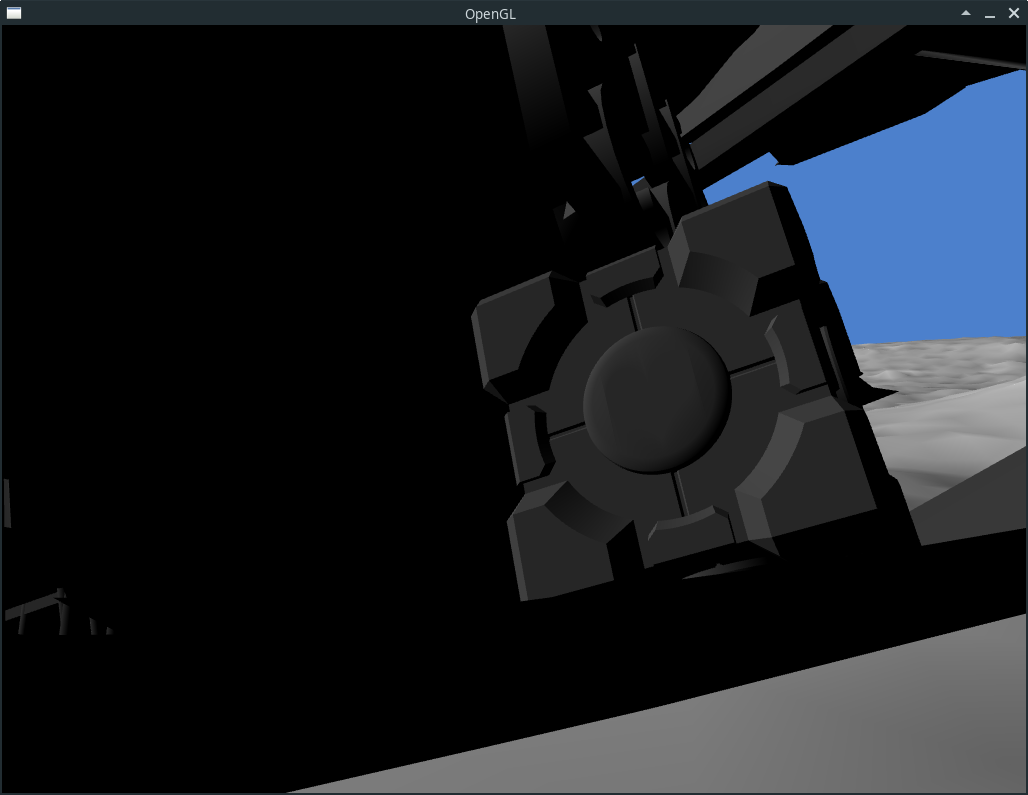
\includegraphics[width=1.00\textwidth]{figures/task7e}
	\caption{Easter egg!}
\label{fig:task7e}
\end{figure}

\subsection{f)}
Extra features (I don't \textit{really} think certain of these deserve extra points, but will list for fun and completeness)

Press SPACE to make the doors open and close again. 

Press C for a \textit{cursed} amount of extra work... Feel free to add any \textit{cursed} music, for atmosphere. My \href{https://www.youtube.com/watch?v=eY52Zsg-KVI}{favourite}.
